\procTitle{История развития геокриологических и гидрологических стационаров Магаданской области}
\procAuthor{Землянскова~А.\,А., Нестерова~Н.\,В.}
\procEmail{anastasiazemlanskova@gmail.com}
\procOrganization{СВНИМС ИМЗ СО РАН} \procCity{Магадан}

\makeProcTitle
\index{z@Землянскова~А.\,А.}
\index{n@Нестерова~Н.\,В.}

Одним из основных факторов, влияющих на процессы формирования стока Восточной Сибири, является мерзлота. Тесная взаимосвязь потоков воды и тепла в речных бассейнах обуславливает значительную чувствительность системы к климатическим и антропогенным изменениям. Отсутствие современных данных о процессах формирования стока в условиях распространения многолетней мерзлоты является острой проблемой для труднодоступных горных районов Восточной Сибири.

На территории Магаданской области расположены уникальные научные стационары с~длительным рядом гидрологических и криогенных наблюдений. Среди них~--- Колымская водно-балансовая станция (КВБС) и стационар Анмангындинской наледи (см.~рис.).

\begin{figure}[h!]
\begin{changemargin}{-1.25cm}{0cm}
  \begin{center}
    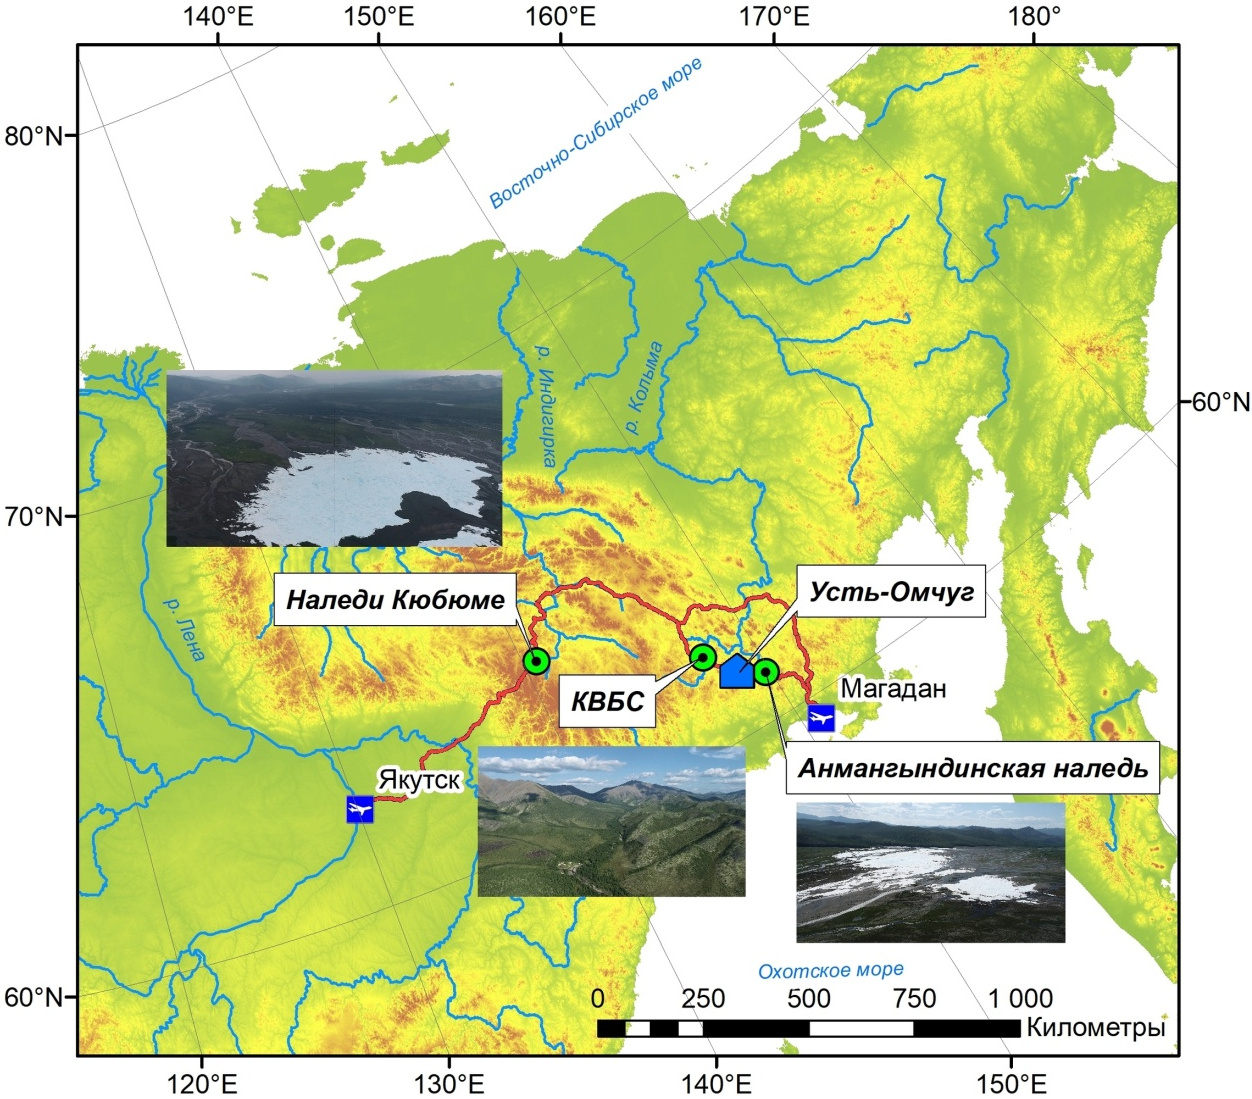
\includegraphics[width=1.2\textwidth]{authors/zemlaykova-2-fig.jpg}
  \end{center}
\end{changemargin}
  \caption*{\textbf{Уникальные научные стационары Северо-Востока России}}
  \label{fig:zemlaykova-2-fig}
\end{figure}


\textbf{Колымская водно-балансовая станция (КВБС)}. Колымская водно-балансовая станция является научным наследием и предметом национальной гордости России, не имеющим аналогов в мире. Возобновление непрерывных наблюдений и исследований на Колымской станции сейчас являются как нельзя более актуальной задачей ввиду повышенного интереса к~природным процессам Арктики и возможностью освоения богатых природных ресурсов Восточной Сибири.

Колымская водно-балансовая станция (КВБС) располагается в верховьях р.~Колымы, в горной местности (перепад высот 830--1690~м), в зоне сплошного распространения многолетней мерзлоты. Среднемноголетняя температура воздуха составляет около $-$12\,\dgС, а количество осадков~--- от~250 до~440~мм в год. Большая часть территории покрыта каменными осыпями, зарослями кедрового стланика и лиственничным редколесьем. Мощность многолетнемерзлых пород достигает 400~м, глубина летнего протаивания составляет от 20~см в~заболоченных низинах до 3~м в гольцах. Условия формирования и характеристики стока на станции являются репрезентативными для обширной территории Верхней Колымы и~прилегающих к~ней районов Северо-Востока России.

Станция была заложена 15 октября 1947~г. гидрометеорологической службой Дальстроя. Инициаторами открытия станции были начальник Гидрометслужбы Дальстроя~Л.~Н. Морозов и начальник научно-ис\-сле\-до\-ва\-тель\-ско\-го отдела А.~Г.~Левин [4]. Первоначальной целью организации станции являлось изучение процессов формирования стока малых рек в~условиях горно-таежного ландшафта и распространения многолетнемерзлых пород, характерных для Северо-Востока СССР.

Уже в мае 1948~г. начались первые наблюдения за стоком воды на ручьях Контактовый (21,2~км$^2$) и Встреча (5,35~км$^2$), а также регулярные наблюдения на метеорологической площадке <<Нижняя>>. В 1957~г. станция перешла в ведение Колымского управления Гидрометслужбы. Программа наблюдений с каждым годом расширялась, охватывая самые удалённые и~труднодоступные уголки станции. В 1960~г. начались наблюдения за стоком воды на руч.~Южном, продолжалась рационализация осадкомерной сети, установлены радиоосадкомеры. В 1963~г. задействованы две дополнительные воднобалансовые площадки.

В 1968~г. начаты измерения стока на уникальном объекте, в бассейне руч.~Морозова, который полностью лишён растительного покрова и сложен каменными осыпями. Проводились экспериментальные исследования по изучению влияния внутригрунтовой конденсации на сток воды с использованием оригинальных приборов и установок. Коллектив станции составлял около 30 человек с профессиональным высшим или средним образованием.

В 1969~г. Колымская стоковая станция переименована в Колымскую водно-балансовую станцию (КВБС). В эти годы осуществлён переход к широким экспериментальным наблюдениям водного баланса во всех его звеньях, к повышению технического уровня исследований [2]. В 1976~г. станцию посетила делегация американских учёных. Они высоко оценили профессиональные и личностные качества работников станции, их преданность делу, которые являлись основой для масштабных полевых и теоретических работ, несмотря на простоту имевшегося оборудования и суровые условия жизни. По мнению Slaughter и Bilello [9], материалы, полученные на КВБС, не имели аналогов в мировой практике.
\clearpage
С начала 1990-х~гг. началось постепенное сокращение программы наблюдений на станции, а с 1997~г. водно-балансовые наблюдения на КВБС законсервированы. Одна метеорологическая станция и пять гидрологических постов действовали на КВБС до июня 2013~г., когда сильный паводок разрушил четыре гидрологических поста. На сегодняшний день там ведутся только стандартные наблюдения на метеорологической площадке и на гидрологическом посту Контактовый~--- Нижний.

Всего с 1948 по 1997~гг. на КВБС действовали десять гидрологических постов на водосборах площадью от 0,27~км$^2$ до 21,6~км$^2$, две метеорологических площадки, 55~осадкомерных пунктов, более 20~мерзлотомеров, несколько гидрогеологических скважин, испарительных, воднобалансовых и стоковых площадок, проводились регулярные снегомерные съемки и~экспериментальные исследования частных гидрологических и мерзлотных процессов [1, 2, 6]. Материалы станции систематизированы и подробно описаны в работе Makarieva et~al. [8].

В отличие от других северных стран, в России в настоящее время нет ни~одного постоянно действующего гидрологического стационара в криолитозоне, который бы проводил целенаправленные исследования гидрологических процессов на водосборах зоны многолетней мерзлоты на постоянной основе, тогда как в Канаде, на Аляске и в Северной Европе действуют не менее двух десятков научно-исследовательских водосборов. Современные данные, продолжающие ряды исторические ряды наблюдений КВБС, могли бы стать ценным индикатором изменений климата и основой для изучения их влияния на состояние мерзлоты и гидрологический режим рек, позволяя заглянуть в механизмы происходящих процессов.

\textbf{Анмангындинская наледь}. Наледи являются элементами водной системы криолитозоны Северо-Востока. Их количество достигает более 7000. Их возникновение связано с~разгрузкой как подземных, так и поверхностных вод, поэтому в зависимости от типа питающих вод реакция наледей на изменение климата различна. В последние десятилетия отмечается изменчивость процессов наледеобразования в различных природно-климатических условиях арктической зоны. Несмотря на работы по исследованию отдельных наледей в~Центральной и Южной Якутии [7], в настоящее время режимные междисциплинарные наблюдения за наледными процессами практически отсутствуют как в России, так и в мире.


Анмангындинская наледь расположена в бассейне р.~Анмангында в районе 155--159~км Тенькинской трассы (Магаданская обл.) в 30~км к юго-востоку от пос.~Усть-Омчуг. Высоты водосбора р.~Анмангында варьируются от 700 до 1850~м. Территория исследования характеризуется суровой зимой и коротким летом. Средняя температура воздуха в июле и~в~январе на м/с~Усть-Омчуг составляет +10,7\,\dgc  и $-$27,7\,\dgc соответственно (1966--2012~гг.). Абсолютный минимум достигает $-$58\,\dgС. Среднегодовая сумма осадков составляет 375~мм (м/с~Усть-Омчуг). Район относится к зоне сплошной многолетней мерзлоты, иногда прерывающейся в таликовых зонах. Мощность многолетнемерзлых пород достигает 200~м, увеличивается на водораздельных участках и снижается в речных долинах [3].

В 1962~г. на базе Колымского УГМС были организованы стационарные исследования режима наледи в бассейне р.Анмангында с целью изучения вопросов регулирования запасов и стока наледных вод.

Основными задачами программы были измерение стока с бассейна, изучение динамики роста и таяния наледного тела, изучение характера влияния климатических факторов на~процессы образования, роста и разрушения наледи. В состав работ входило определение размеров наледи и вычисление объёма льда; картирование наледи и фиксация ледовых образований; изучение процессов формирования стока и влияния климатических факторов на режим наледи; изучение гидрохимического состава поверхностных вод [3, 5].
\clearpage
Работы прекратились в 1992~г. По опросам местных жителей за последние 30 лет происходят заметные изменения в режиме формирования и разрушения наледи. Водосбор р.~Анмангында является репрезентативным для~территории Северо-Востока России, а Анмангындинская наледь является единственным объектом в мире с продолжительным рядом наблюдений за~процессами наледообразования, в том числе динамикой площади и объёма наледного льда.

Перечисленные станции являются научным наследием и предметом национальной гордости России, не имеющим аналогов в мире. Возобновление непрерывных наблюдений и~исследований сейчас являются как нельзя более актуальной задачей ввиду повышенного интереса к природным процессам Арктики и возможностью освоения богатых природных ресурсов Северо-Востока.

\begin{thebibliography}{99}
\bibitem{}\BibAuthor{Банцекина~Т.~В.} Температурный режим и динамика льдистости крупнообломочных склоновых отложений без заполнителя в весенне-летнее время (на~примере руч. Контактовый) // Колыма.~--- 2002.~--- №~4.~--- С.~9--13.
\bibitem{}\BibAuthor{Бояринцев~Е.~Л., Сербов~Н.~Г., Попова~Н.~И.} Формирование водного баланса весеннего половодья малых горных водосборов Верхней Колымы (по материалам Колымской водно-балансовой станции) // Вестник СВНЦ ДВО РАН.~--- 2006.~--- №~4.~--- C.~12--19.
\bibitem{}\BibAuthor{Букаев~Н.} Основные закономерности режима гигантских наледей в верховьях р.Колыма (на~примере Анмангындинской наледи) // Колыма.~--- 1966.~--- №~4.~--- С.~9--12
\bibitem{}Информационное письмо №~2\,(114) 40-летие Колымской Водно-Балансовой станции.~--- Магадан~:  Колымское~ТУГ, 1988.
\bibitem{}\BibAuthor{Лебедев~В., Ипатьева~А.} Анмангындинская наледь, ее режим и роль в водном балансе речного бассейна // Труды ДВНИГМИ. Гидрологические исследования и прогнозы.~--- Л.~: Гидрометеоиздат, 1980.~--- Вып.~84.~--- С.~86--93
\bibitem{}\BibAuthor{Сущанский~С.~И.} История создания, методы, объекты и некоторые результаты исследований Колымской водно-балансовой станции // Факторы формирования общего стока малых горных рек в Субарктике (по~материалам Колымской водно-балансовой станции).~--- Магадан~: СВКНИИ ДВО РАН, 2002.~--- С.~18--35
\bibitem{}\BibAuthor{Gagarin~L., Qingbai~W., Melnikov~A., Volgusheva~N., et al.} Morphometric analysis of groundwater icings: Intercomparison of estimation techniques // Remote Sensing.~--- 2020.~--- Vol.~12~(4).~--- P.~692.~--- DOI:~10.3390/rs12040692.
\bibitem{}\BibAuthor{Makarieva~O., Nesterova~N., Lebedeva~L., Sushansky~S.} Water balance and hydrology research in~a~mountainous permafrost watershed in upland streams of~the Kolyma River, Russia: a database from the Kolyma Water-Balance Station, 1948–1997 // Earth Syst. Sci. Data.~--- 2018.~--- Vol.~10.~--- P.~689--710.~--- DOI:~10.5194/essd-10-689-2018.
\bibitem{}\BibAuthor{Slaugher~C.~W., Billelo~M.~A.} Kolyma Water Balance Station, Magadan oblast, Northeast U.S.S.R. // United Station~--- Soviet Scientific Exchange Visit / Special Report 77--155, Army Cold Regions Recearch and Engineering Laboratory.~--- Hanover~: CRREL, 1977.~--- 66~p.
\end{thebibliography}
